%%%% Paramétrage du TD %%%%
\def\xxactivite{Colle 01 \ifprof -- Corrigé \else \fi} % \normalsize \vspace{-.4cm}
\def\xxauteur{\textsl{Xavier Pessoles}}


\def\xxtitreexo{Porte-outil}
\def\xxsourceexo{\hspace{.2cm} \footnotesize{}}
\def\xxauteur{\textsl{Xavier Pessoles}}


\def\xxcompetences{%
\vspace{.25cm}
\textsl{%
\textbf{Savoirs et compétences :}
\begin{itemize}[label=\ding{112},font=\color{ocre}] 
\item \textit{C2-08} :Déterminer les actions mécaniques en dynamique dans le cas où le mouvement est imposé.
\end{itemize}
}}
\def\xxfigures{
%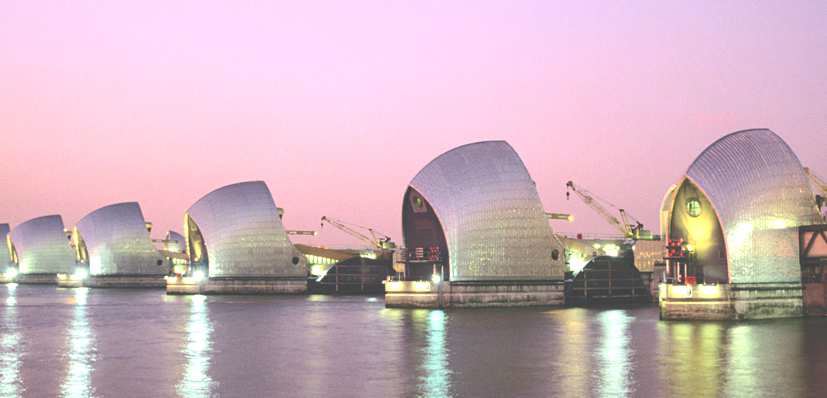
\includegraphics[width=.7\linewidth]{fig_00}
}%figues de la page de garde


\input{\repRel/Style/pagegarde_TD}
\setcounter{numques}{0}

\setlength{\columnseprule}{.1pt}

\pagestyle{fancy}
\thispagestyle{plain}

\vspace{5.1cm}

\def\columnseprulecolor{\color{ocre}}
\setlength{\columnseprule}{0.4pt} 

%%%%%%%%%%%%%%%%%%%%%%%

\setcounter{exo}{0}

\ifprof
\else
\begin{multicols}{2}
\fi

Le dispositif porte-outil d'une machine d'affûtage est composé de trois solides \textbf{1}, \textbf{2} et \textbf{3}. 

\begin{center}
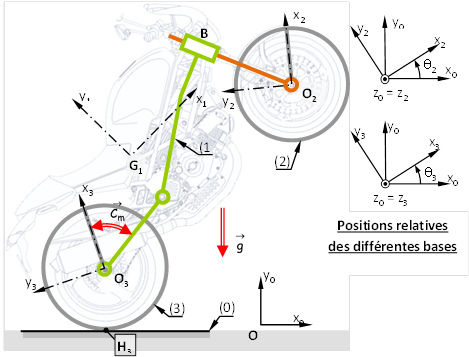
\includegraphics[width=\linewidth]{fig_01}
\end{center}
Le repère $\mathcal{R}_0=\repere{O}{x_0}{y_0}{z_0}$, avec $\axe{O}{\vect{z_0}}$ vertical ascendant, est lié au bâti \textbf{0} de la machine. Il est supposé galiléen. Toutes les liaisons sont supposées parfaites.

Le repère $\mathcal{R}_1=\repere{O}{x_1}{y_1}{z_0}$ est lié au support tournant \textbf{1} en liaison pivot d'axe $\axe{O}{z_0}$ avec le bâti \textbf{0}. La position de \textbf{1} par rapport à l'axe $\axe{O}{z_0}$ est repérée par $\alpha=\angl{x_0}{x_1}=\angl{y_0}{y_1}$. 

On note $I_1$ le moment d'inertie de \textbf{1} par rapport à l'axe $\axe{O}{z_0}$ et $H$ le point tel que $\vect{OH}=h{x_1}$.

Le repère $\mathcal{R}_2=\repere{H}{x_2}{y_1}{z_2}$ est lié au bras pivotant \textbf{2} en liaison pivot d'axe $\axe{H}{\vect{y_1}}$ avec \textbf{1}. La position de \textbf{2} est repérée par $\beta=\angl{x_1}{x_2}=\angl{z_0}{z_2}$. 

On note $m_2$ la masse de \textbf{(2)}, de centre d'inertie $H$ de matrice d'inertie $\inertie{H}{2}=\matinertie{A_2}{B_2}{C_2}{0}{0}{0}{\mathcal{R}_2}$.

Le repère $\mathcal{R}_3=\repere{G}{x_3}{y_3}{z_2}$ est lié au porte-outil  \textbf{(3)} (avec l'outil à affûter tenu par le mandrin) en liaison pivot glissant d'axe $\axe{H}{z_2}$ avec \textbf{(2)}. 

La position de \textbf{(3)} est repérée par $\gamma=\angl{x_2}{x_3}=\angl{y_2}{y_3}$ et par $\vect{HG}=\lambda\vect{z_2}$. 

On note $m_3$ la masse de \textbf{(3)}, de centre d'inertie $G$ de matrice d'inertie $\inertie{G}{3}=\matinertie{A_3}{B_3}{C_3}{0}{0}{0}{\mathcal{R}_3}$.

\question{Justifier la forme de la matrice de la pièce~\textbf{(3)}.}

\question{Calculer $\vectv{G}{3}{0}$.}

\question{Indiquer la méthode permettant de calculer le torseur dynamique en $G$ de \textbf{(3)} en mouvement par rapport à $\mathcal{R}_0$ en projection sur $\vect{z_2}$.}

\question{Calculer le moment  dynamique en $H$ appliqué à l'ensemble \textbf{\{2, 3\}} en mouvement par rapport à $\mathcal{R}_0$ en projection sur $\vect{y_1}$.}

\question{Calculer le moment dynamique en $O$ appliqué à l'ensemble \textbf{\{1, 2, 3\}} en mouvement par rapport à $\mathcal{R}_0$ en projection sur $\vect{z_0}$.}


\ifprof
\else
\end{multicols}
\fi

\ifprof
\begin{enumerate}
\item $\torseurcin{V}{3}{\mathcal{R}_0}=\torseurl{\dot{\alpha}\vect{z_0}+\dot{\beta}\vect{y_1}+\dot{\gamma}\vect{z_2}}{r\dot{\beta}\vect{x_2}+\left( h+r\sin \beta \right)\dot{\alpha}\vect{y_1}+\dot{r}\vect{z_2}}{G}$.
\item $\vectg{G}{3}{\mathcal{R}_0}=$
$\left(2\dot{r}\dot{\beta}+r\ddot{\beta} \right)\vect{x_2}$

$\quad +\left[2\dot{\alpha}\left( \dot{r}\sin\beta +r\dot{\beta} \cos \beta \right) + \left(h+r\sin\beta \right)\ddot{ \alpha}\right]\vect{y_1}$

$\quad -\left(h+r\sin\beta \right)\dot{\alpha}^2\vect{x_1}$

$\quad +\left(\ddot{r}-r\dot{\beta}^2 \right)\vect{z_2}$.
\end{enumerate}
\else
\fi

\newpage

\ifprof
\begin{center}
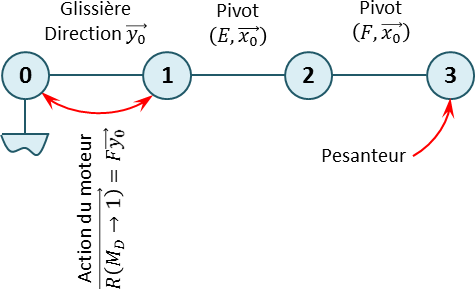
\includegraphics[width=\linewidth]{cor_01}
\end{center}
\begin{center}
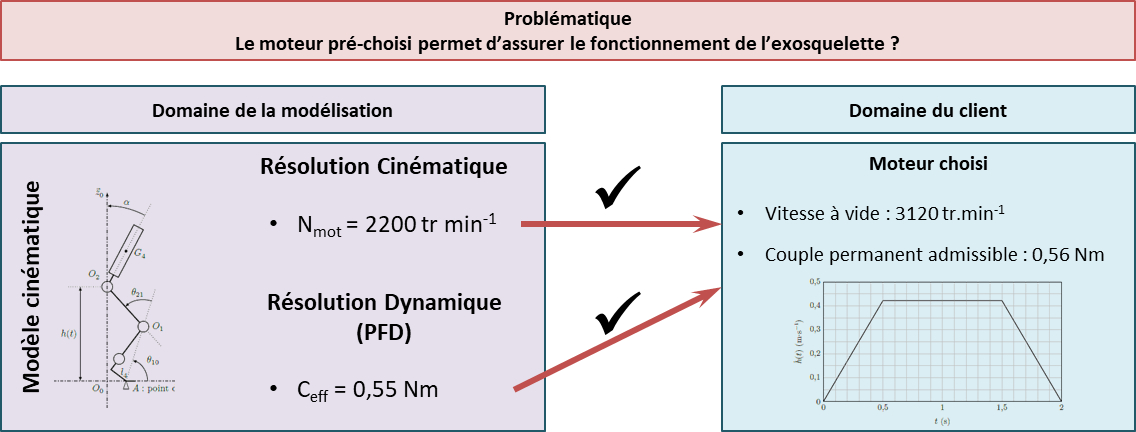
\includegraphics[width=\linewidth]{cor_02}
\end{center}
\begin{center}
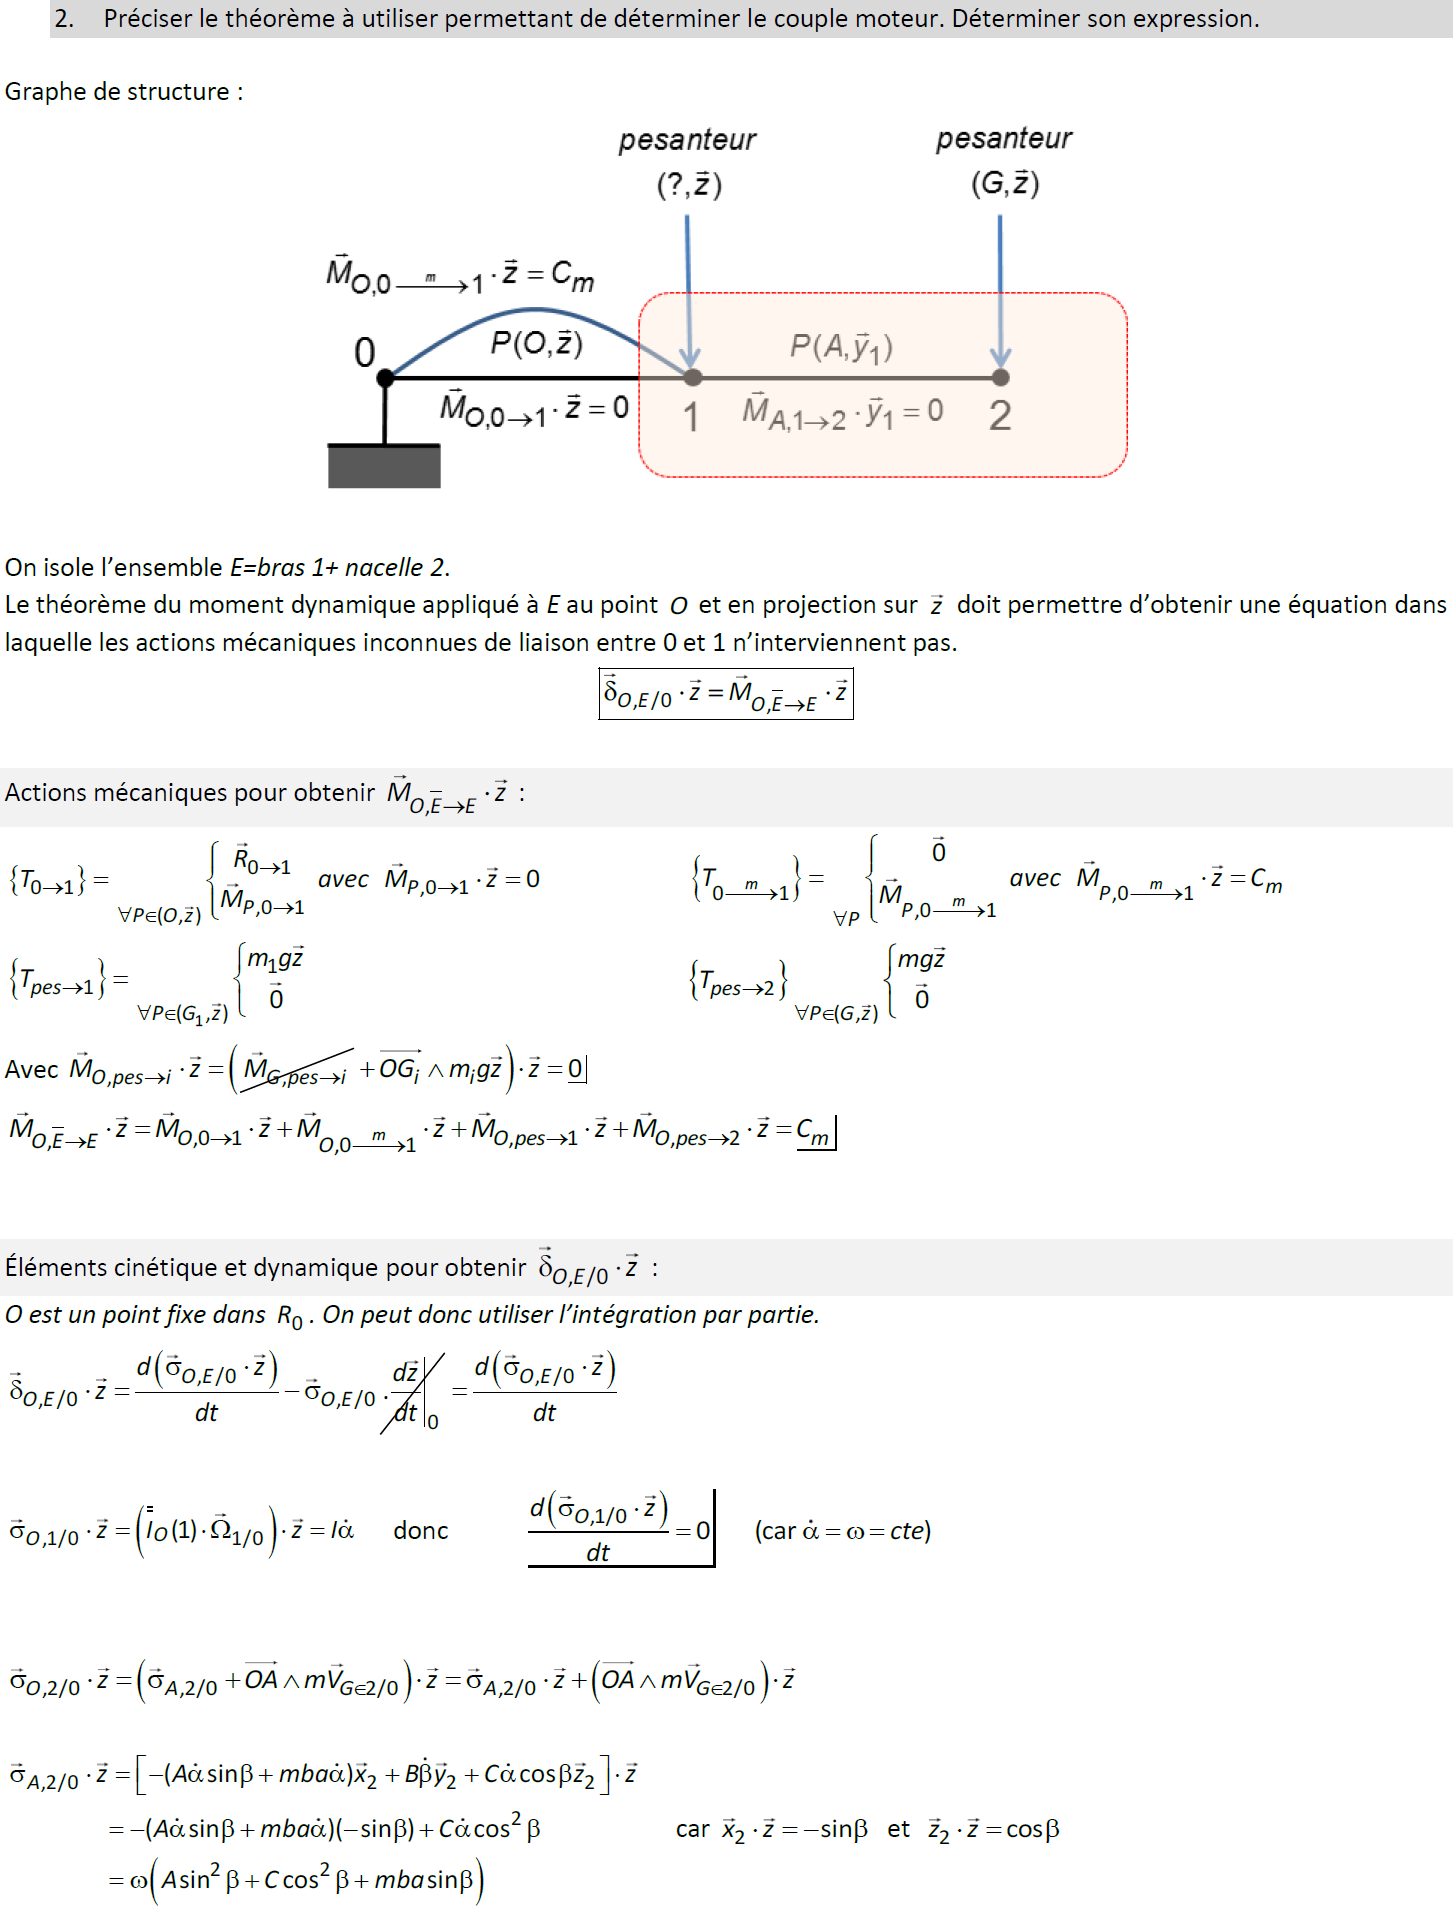
\includegraphics[width=\linewidth]{cor_03}
\end{center}
\begin{center}
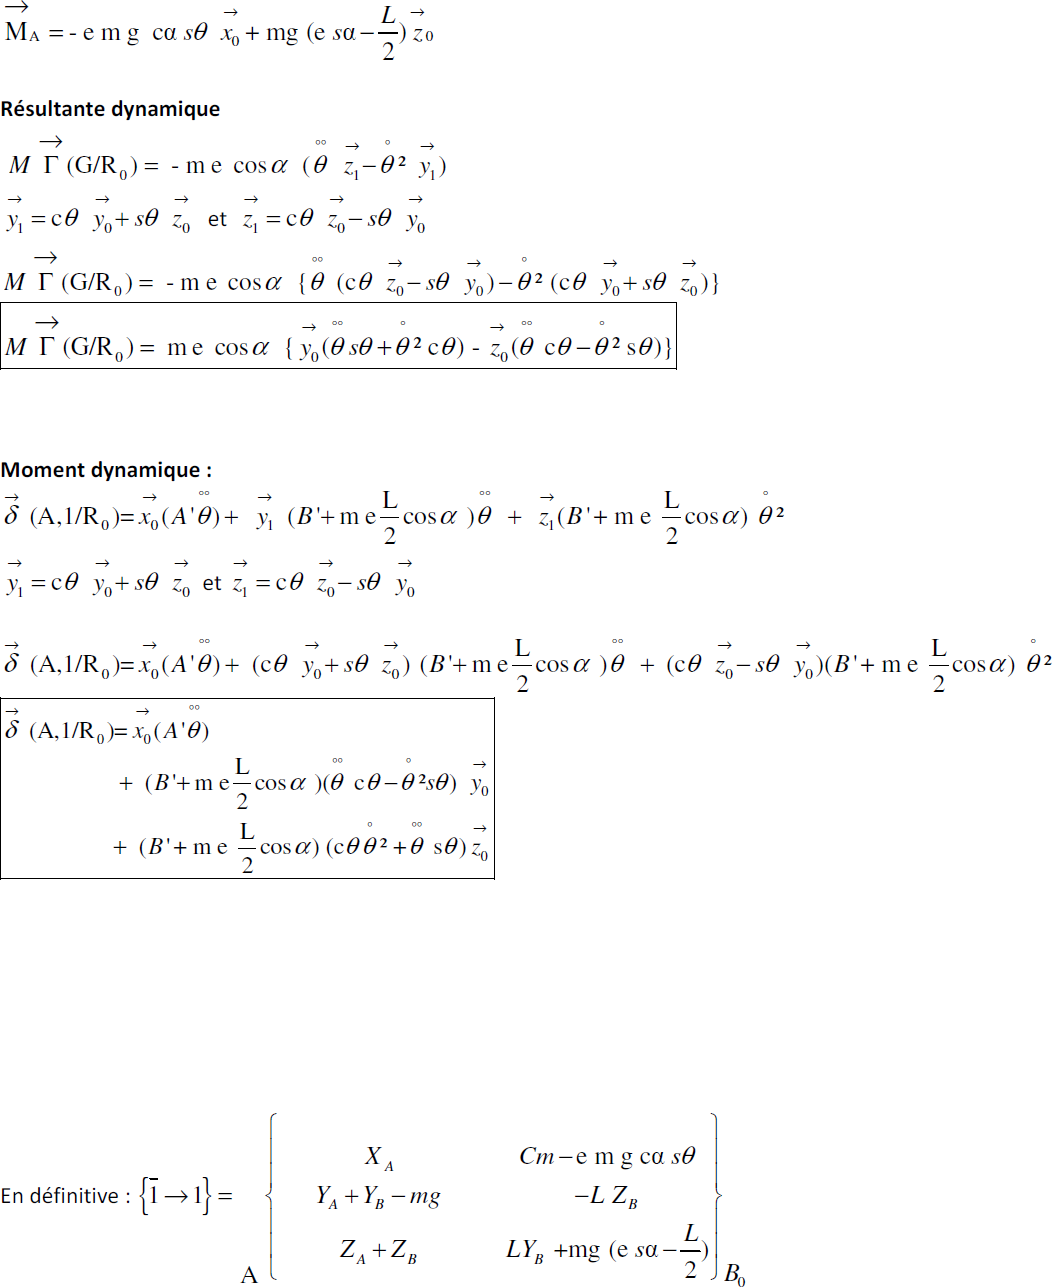
\includegraphics[width=\linewidth]{cor_04}
\end{center}
\begin{center}
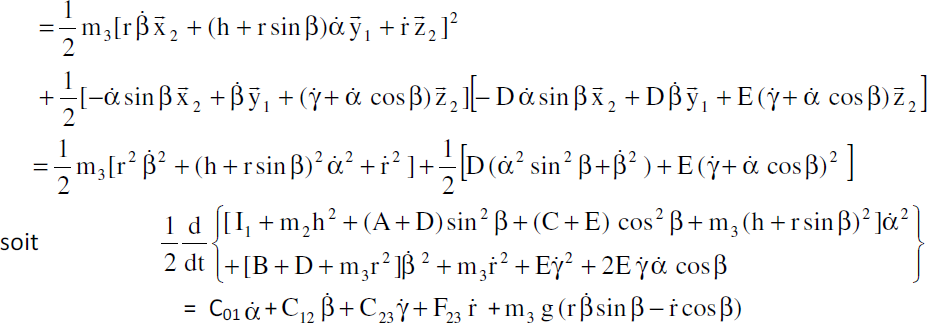
\includegraphics[width=\linewidth]{cor_05}
\end{center}
\else
\fi

%\newpage

